\documentclass{article}
\usepackage{fullpage}
\usepackage{parskip}
\usepackage{hyperref}
\usepackage{listings}
\usepackage{graphicx}
\usepackage{amssymb}
\usepackage{mdwlist}
\usepackage{textcomp}
\usepackage[usenames,dvipsnames]{color}
\hypersetup{
    colorlinks,
    citecolor=Red,
    linkcolor=Red,
    urlcolor=Red}
\begin{document}

\title{Assignment 3: Textures}
\author{CS148 Fall 2015-2016}
\date{}
\maketitle

\section*{Introduction}

\begin{figure}[h!]
    \centering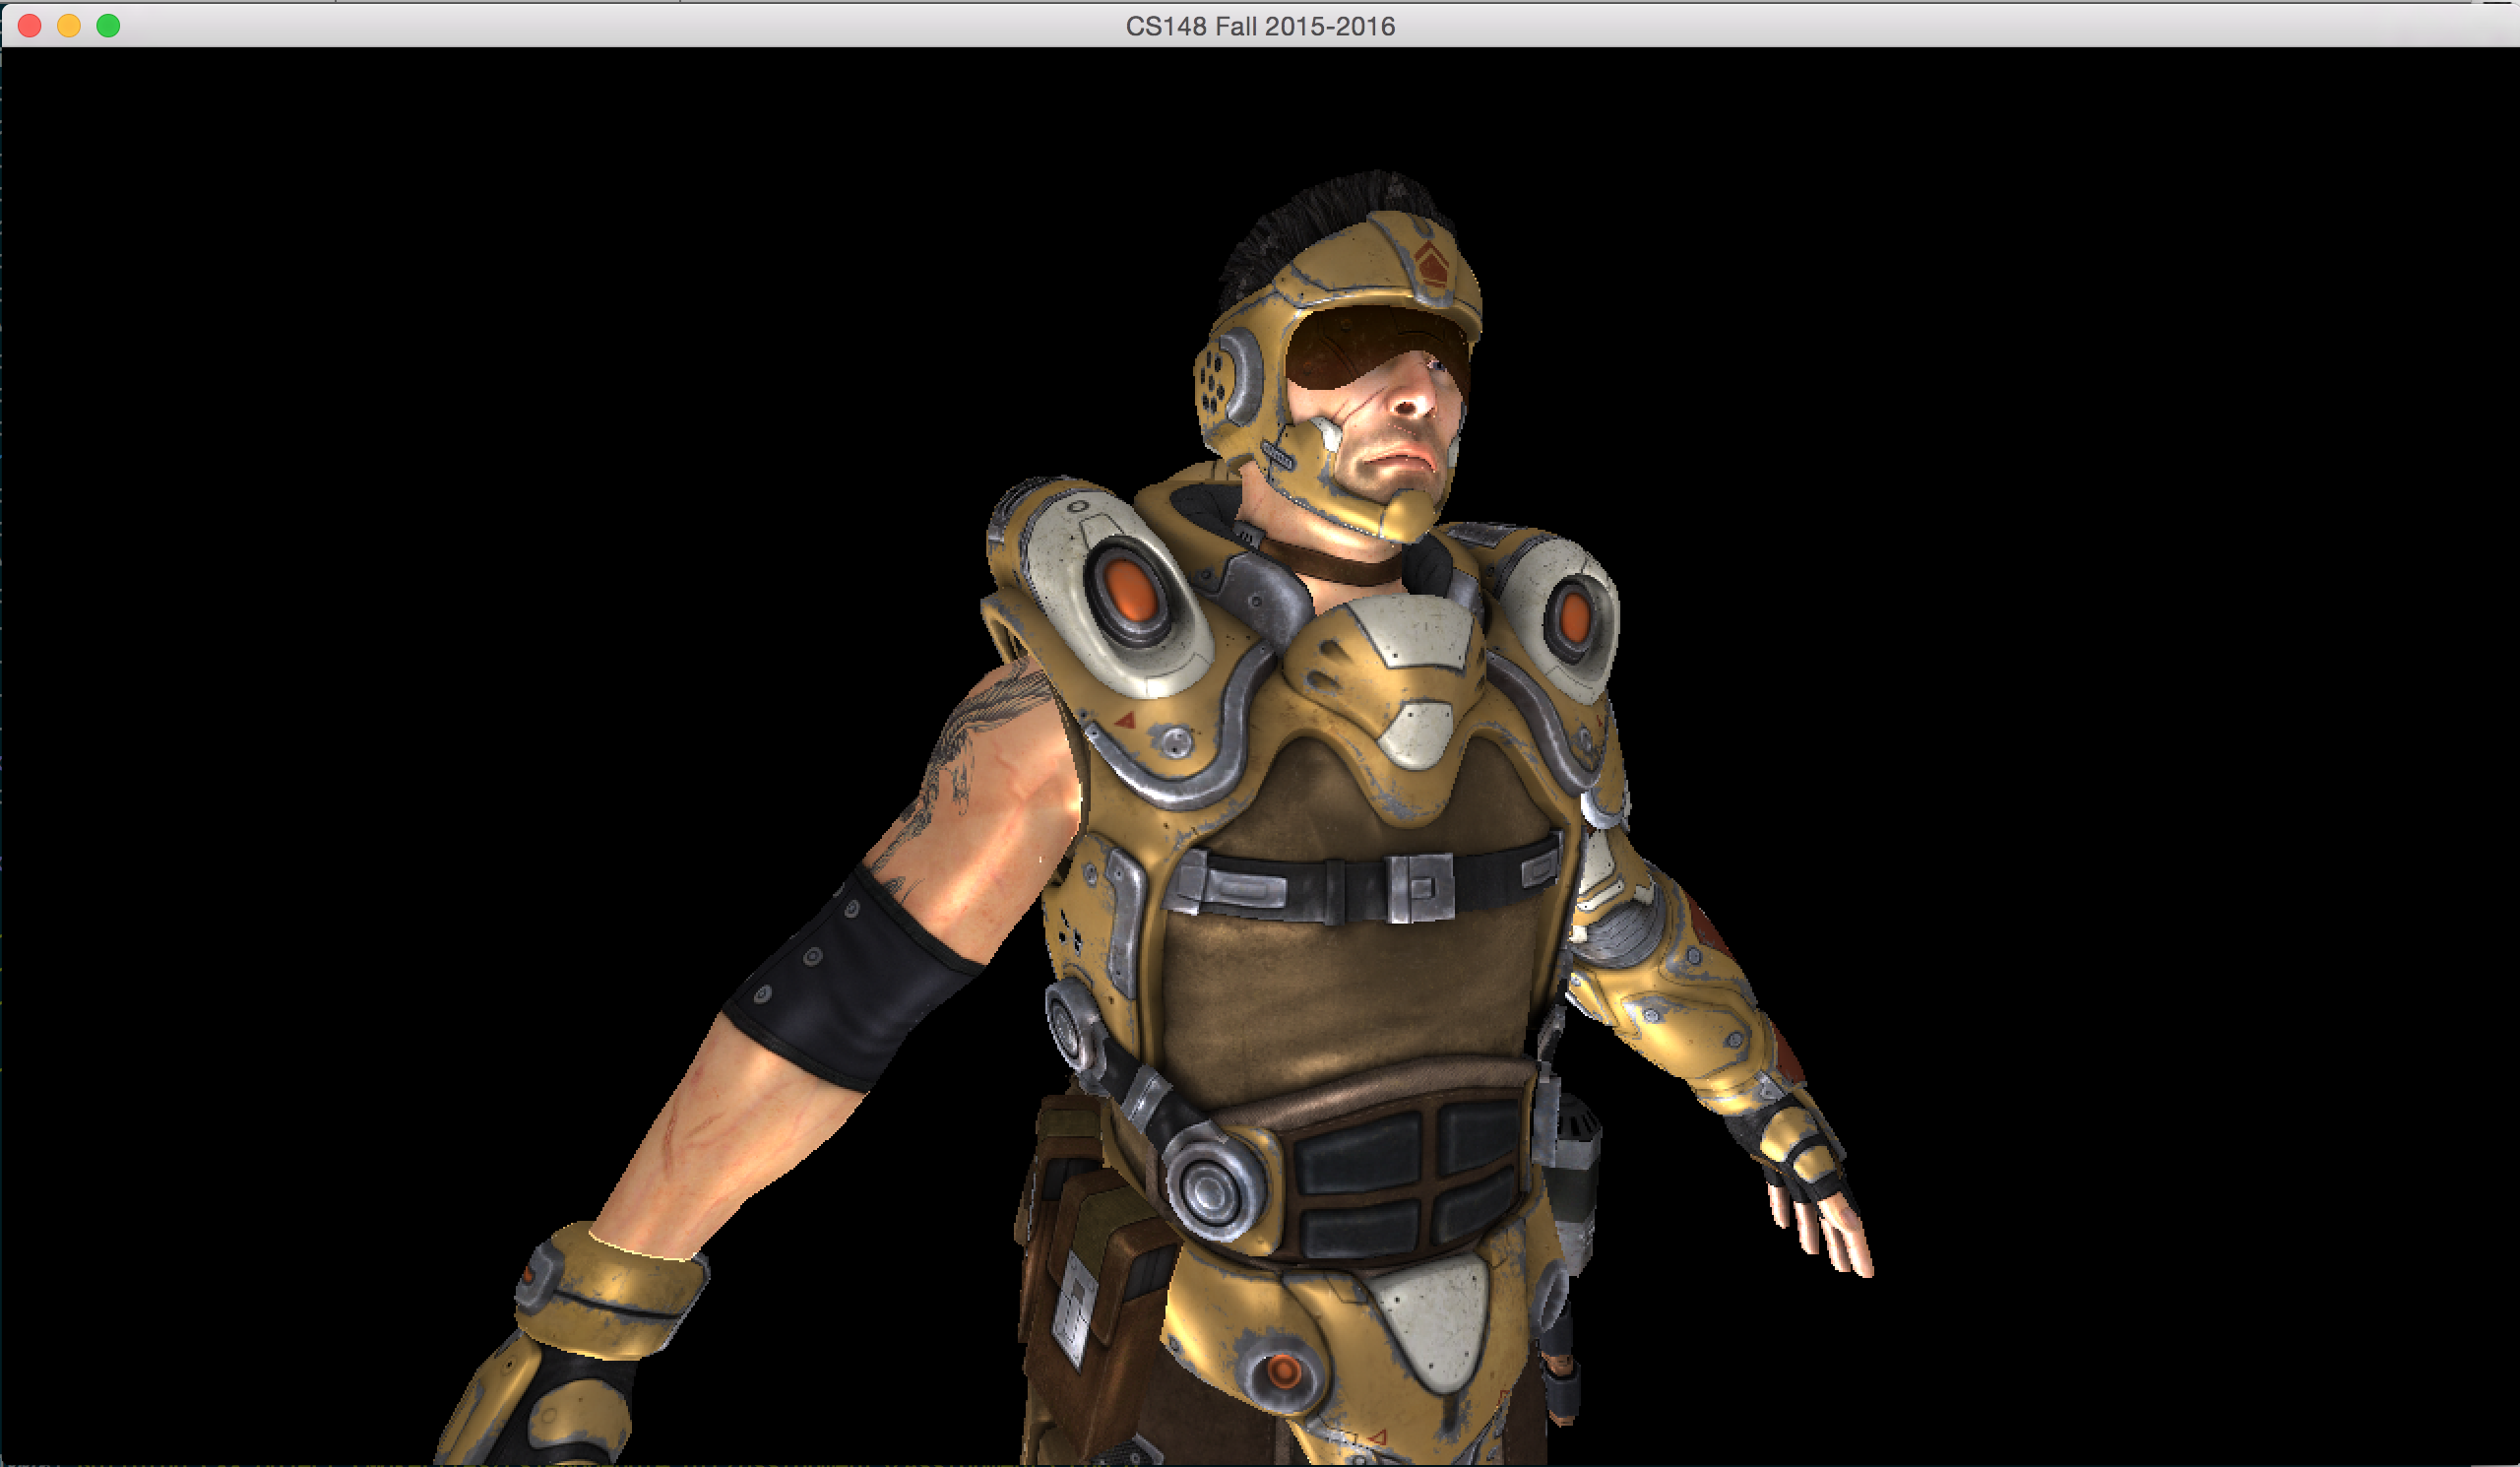
\includegraphics[width=0.7\linewidth]{assign3.png}
    \caption{A 3D model with difuse and specular textures.}
\end{figure}

This assignment will build upon the previous assignment to also incorporate textures. In the provided assignment framework, we show you how to use a diffuse and specular texture to perform Blinn-Phong shading. You will expand upon this to implement normal mapping which allows relatively low-poly meshes to look like they have a lot of detail on them. Textures are commonly used to make low-poly models look much more realistic, especially in video games where it is cheaper (to a point) to render a high quality texture on a low-poly mesh than a normal-quality texture on a high-poly mesh. Remember, start early and ask questions if you get stuck!

Throughout the assignment, you should also go back to the scene you setup in assignment 2 and start texturing it to submit as your final image.

\subsection*{Useful Resources}

\begin{enumerate*}
    \item OpenGL Programming Guide Chapter 6 (the book is not required, but recommended!)
    \item OpenGL 4 Documentation: \href{https://www.opengl.org/sdk/docs/man4/}{here}. Note that these pages are for OpenGL 4.5 but most should be equivalent (unless otherwise noted on the function's page).
    \item SDL 2 Documentation: \href{https://wiki.libsdl.org/CategoryAPI}{here}.
    \item GLSL Tutorial: \href{http://www.lighthouse3d.com/tutorials/glsl-tutorial/}{here}.
    \item GLM: \href{http://glm.g-truc.net/0.9.7/glm-0.9.7.pdf}{Manual} and \href{http://glm.g-truc.net/0.9.7/api/index.html}{Documentation}.
    \item C++ Reference: \href{http://en.cppreference.com/w/}{here}
    \item Open Asset Import Library Documentation: \href{http://assimp.sourceforge.net/lib_html/index.html}{here}
    \item FreeImage Manual: \href{http://downloads.sourceforge.net/freeimage/FreeImage3170.pdf}{here}.
    \item Assignment Framework Documentation: This can be found in "source/doxygen"
\end{enumerate*}

\subsection*{UVs and Textures}

How does a particular vertex know which pixel from the texture to use? The answer to that is via UV Mapping (\href{https://en.wikipedia.org/wiki/UV_mapping}{Wikipedia}). Each vertex is given a UV coordinate (usually you do this in your modeling software of choice, see below) which ranges from (0, 0) (bottom left corner) to (1, 1) (top right corner). Then in the vertex/fragment shader, the a texture is sampled from that coordinate to get some values which can be interpreted as anything! For the diffuse and specular textures we choose to interpret the texture values as colors.

To create UV's, you can follow a tutorial for your modeling software. For Maya, a good tutorial can be found \href{https://www.youtube.com/watch?v=HLhazEa8wmw}{here}. Look around on Youtube, there are plenty of tutorials for you to follow!

\section*{Assignment}

\subsection*{Assignment 3 Code Explanation}

Look in the Assignment3 class documentation in the assignment framework documentation found at "source/doxygen".

\subsection*{Provided Asset}

You may have noticed that we have provided you a model courtesy of Marcus Dublin on Polycount. You can find the original model thread here: \href{http://www.polycount.com/forum/showpost.php?p=1589706&postcount=68}{link}. This model comes in three parts, the body, backpack, and head/arms which can be found in "assets/outlander/Model". Additionally, this model also comes with textures found in "assets/outlander/TGA". In the assignment 3 source code, you can see how we are using the diffuse and the specular textures. There are also other textures provided, for example: glow, normal, and alpha. For this assignment, it is only mandatory to implement the normal map, but feel free to also incorporate the other textures as well!

\subsection*{Pointers to Get You Started}
\begin{itemize*}
    \item This \href{http://www.opengl-tutorial.org/intermediate-tutorials/tutorial-13-normal-mapping/}{link} will be very helpful to understand how normal mapping works. The bottom of this link also has some nice links to help you generate normal maps! Additionally the \href{https://en.wikipedia.org/wiki/Normal_mapping}{Wikipedia} page may help as well.
\end{itemize*}

\subsection*{Going Further (Optional)}
\begin{itemize*}
    \item Sky boxes are a great way to fill up your background with something rather than a single color. It is what it sounds like. You render a giant box and slap a texture on it. Sky box! You can look at this \href{http://ogldev.atspace.co.uk/www/tutorial25/tutorial25.html}{tutorial} to get started. A more general tutorial for cube mapping can be found \href{http://learnopengl.com/#!Advanced-OpenGL/Cubemaps}{here}. This \href{http://answers.unity3d.com/questions/33102/where-can-i-download-skyboxes.html}{link} has some useful links to find skybox textures to download.
\end{itemize*}

\section*{Feedback (Optional)}
\begin{enumerate*}
    \item On a scale of 1-10 [10 being the most work]: How much work was this assignment?
\end{enumerate*}

\section*{Grading}
This assignment will be graded on the following requirements
\begin{itemize*}
    \item There are at least two different geometric models in your scene.
    \item At least two models have a diffuse texture, specular texture, and a normal texture.
    \item Normal mapping is implemented correctly.
\end{itemize*}
according to the following rubric.
\begin{itemize*}
\item $+$ -- Exceeds the requirements via one or more artistic/technical contributions
\item $\checkmark$ -- Meets all of the requirements
\item $-$ -- Does not meet the requirements but still produces a drawing.
\item $0$ -- The submitted solution does not produce a drawing.
\end{itemize*}

\end{document}

